% !TEX TS-program = pdflatex
% !TEX encoding = UTF-8 Unicode

% Matthew Urffer Master Thesis
% 

%%%%%%%%%%%%%%%%%%%%%%%%%%%%%%%%%%%%%%%%%%%%%%%%%%%%%%%%%%%%%%%%%%%%%%%%%%%%%%%
% 																							         %
%					                         PREAMBLE      								%
%																										%
%%%%%%%%%%%%%%%%%%%%%%%%%%%%%%%%%%%%%%%%%%%%%%%%%%%%%%%%%%%%%%%%%%%%%%%%%%%%%%%
\documentclass[compress]{beamer}

\mode<presentation>
{
  %\usetheme{Boadilla}
  \usetheme{Frankfurt}
  \usecolortheme{crane}
  \setbeamercovered{transparent}
}

% Package Setup
\usepackage[english]{babel}
\usepackage[utf8]{inputenc}
\usepackage{times}
\usepackage[T1]{fontenc}
\usepackage{multicol}
\usepackage{array}				% Table Stuff
\usepackage{arydshln}
\usepackage{multirow}
\usepackage{rotating}
\usepackage{graphics}
\usepackage{caption}            % Caption Stuff
\captionsetup{font=scriptsize,labelfont=scriptsize}
\usepackage{amsmath}				% Math Stuff
\usepackage{listings}				% Code Example Stuff
\bibliographystyle{ieeetr}

\lstset{% General Listing Settings
	basicstyle=\tiny,
	frame=single
}


% Preamble / Frst Size
\setbeamersize{text margin left=5mm, text margin right 5mm}
\title[Matthew Urffer Master's Thesis] {Design of a Neutron Detector Capable of Replacing ${}^3$He Detectors Utilizing Thin Polymeric Films}
\subtitle{Master's Thesis Defense}
\author[] {Matthew Urffer\inst{1} }
\institute[University of Tennessee] { 
  \inst{1}%
  Department of Nuclear Engineering\\
  University of Tennessee, Knoxville, TN
}

\date[] {November 8th, 2012}
\pgfdeclareimage[height=0.5cm]{university-logo}{images/utwordmarkhorz.eps}
\logo{\pgfuseimage{university-logo}}


% Delete this, if you do not want the table of contents to pop up at
% the beginning of each subsection:
\AtBeginSection[]
{
  \begin{frame}<beamer>{}
    \frametitle{\insertsectionhead}
    \begin{multicols}{2}
  % \tableofcontents[currentsubsection,hideothersubsections,sectionstyle=show/hide,subsectionstyle=show/shaded,]
    \tableofcontents[currentsection] 
    \end{multicols}
  \end{frame}
}


% If you wish to uncover everything in a step-wise fashion, uncomment
% the following command: 
%\beamerdefaultoverlayspecification{<+->}


\begin{document}

\begin{frame}
  \titlepage
\end{frame}

\begin{frame}{Table of Contents}
  \begin{multicols}{2}
    %\tableofcontents[currentsection,pausesections]
    \tableofcontents[currentsection]
    \end{multicols}
\end{frame}


%%%%%%%%%%%%%%%%%%%%%%%%%%%%%%%%%%%%%%%%%%%%%%%%%%%%%%%%%%%%%%%%%%%%%%%%%%%%%%%
%                                                                             %
%                             START OF CONTENT                                %
%                                                                             %
%%%%%%%%%%%%%%%%%%%%%%%%%%%%%%%%%%%%%%%%%%%%%%%%%%%%%%%%%%%%%%%%%%%%%%%%%%%%%%%
\section{Introduction}

A supervised machine learning problem is one which a learning algorithm is presented a set of training data and attempts to find an unknown function which maps the training values to the correct answer.
Typically the training set, denoted $S$, is a set of the form $\left \{ (\vec{x}_1,y_1), (\vec{x}_2,y_2), \dots, (\vec{x}_n,y_n) \right \}$ where $\vec{x}_i$ is vector of some features of the problem.
Examples of problem features include discrete or real valued items such as height, weight, age, zip code, grade point average, starting salary, and telephone number (as just a few)  which might make up the features of a person.
The $y_i$ are the class of the training feature $\vec{x}_i$ belongs to; these might be University of Tennessee students or Carnegie Mellon students.
In this examples students with a zip code of 15213 are likely to be Tartans, while students with a zip code of 37916 are like to be Volunteers.
The challenge arises from examples have overlapping features; for example this author as a former Tartan and current Vol would be difficult to classify by zip code.
The learning algorithms job is then to find a hypothesis $h$ that correctly classifies a student as a Volunteer of Tartan based on the features provided.
This learning process can then be defined as finding the hypothesis that has the least error (incorrect classifications) on the training data set while extending to examples outside of the training space.

\subsection{Support Vector Machines}
Support Vector Machines (SVM) are a supervised learning technique in which hyperplanes are constructed in a high dimensional space to which the features are mapped.
SVMs find the hyperplanes that are the farthest away from all of mapped features in order to provide excellent training performance while still maintaining the ability to generalize to new instances; i.e. SVMs are maximal margin classifiers.
For a binary classification the decision function of the SVM is the dot product of the weight vector and the training example in the feature space added to a bias vector as shown in Equation \ref{eq:BCSVM}.
\begin{equation}
\label{eq:BCSVM}
f \left ( \vec{x} \right ) = \left \langle \vec{w} \phi(\vec{x}) \right \rangle + \vec{b}
\end{equation}
where $\phi(\vec{x})$ is a mapping to the higher dimensional space.
The SVM is then learning the optimal values of the weight vector $\vec{w}$ and the basis $\vec{b}$.

The radial basis function (Equation \ref{eq:RBF}) is a common kernel function used to map the input vector $\vec{x}$ into a higher dimension.
\begin{equation}
\label{eq:RBF}
k \left ( \vec{x}_i , \vec{x}_j \right ) = exp \left ( - \frac{\left \| \vec{x}_i - \vec{x}_j \right \|}{2\sigma^2} \right ) 
\end{equation}
The maximal margin is ensured by minimizing:
\begin{equation}
\label{eq:Min}
g(\vec{w},\eta) = \frac{1}{2} \left \| \vec{w} \right \| + C \sum_{i=1}^N \zeta_i
\end{equation}
subject to:
\begin{equation}
\label{eq:Constraint}
y_i( \left \langle \vec{w},\phi(\vec{x}) \right \rangle + b ) \ge 1-\zeta_i, ~~~\zeta_i \ge 0
\end{equation}
where $\zeta_i$ is the $i$th slack variable and C is the regularization parameter \cite{li_adaboost_2008}.
This problem can be translated  in to the Wolfe dual form, which can be solved with quadratic programing \cite{li_adaboost_2008}.

\subsection{Boosting}
Unbalanced data sets (data sets in which a majority of the values come from one class, see Figure \ref{fig:ClassDist}) are difficult for classification schemes to learn because the minority class is not well represented and tends to be thought as noise for the classifier.
Often classifiers are trained from unbalanced data sets by artificially balancing the data set by sampling techniques; i.e. up-sampling (sampling more from the minority class) and down-sampling (sampling less from the majority class).
Boosting is an ensemble learning method in which a set of weights is maintained over the training samples and adaptively adjusted after each training iteration according to the ones that are misclassified \cite{li_adaboost_2008}.
Given an individual classifier $h$, an ensemble of classifiers can be constructed of a set of individual classifiers, $H={h_1, h_2,\dot, h_n}$.
By maintaining a weight distribution over all of the training examples, these weights could be updated to emphasize the training examples that are misclassified incorrectly.  These incorrectly classified examples could then be learned in a refinement of the classifier or by training adding a new classifier to the ensemble with the new weights.
Performance of the ensemble is enhanced as long as the individual classifiers are weak and have uncorrelated errors as when any single classifier is incorrect the other classifiers in the ensemble might correctly classify the example.
\begin{figure*}[ht!]
	\centering
	\begin{subfigure}[b]{0.3\textwidth}
		\centering
		\includegraphics[width=\textwidth]{Liver_ClassDist}
        \caption{Liver}
	\end{subfigure}%
	~
	\begin{subfigure}[b]{0.3\textwidth}
		\centering
		\includegraphics[width=\textwidth]{Glass_ClassDist}
        \caption{Glass}
	\end{subfigure}	
    ~
	\begin{subfigure}[b]{0.3\textwidth}
		\centering
		\includegraphics[width=\textwidth]{Vowel_ClassDist}
        \caption{Vowel}
	\end{subfigure}%
	\caption{Distribution of Class Data}
	\label{fig:ClassDist}
\end{figure*}

%%%%%%%%%%%%%%%%%%%%%%%%%%%%%%%%%%%%%
\section{Methods}
\label{sec:Methods}

For convince a subversion repository was created to manage the developed code base, and all source code is available by anonymous checkout from \verb+http://www.murphs-code-repository.googlecode.com/svn/trunk/layeredPolymerTracking+. Revision 360 was the code base used to generate the results shown in \ref{sec:Results}.

\subsubsection{Detector Geometry}
The geometry was setup such that it is possible to define multiple layers of detectors, as shown in Figure \ref{fig:LayerDetectorGeo}.
This was done by creating a 
\begin{figure} 
    \includegraphics[width=\figurewidth]{10LayerGamma}
	\caption{10 Layer Detector with a simulated gamma event}
    \label{fig:LayerDetectorGeo}
\end{figure}
\subsubsection{Physics Lists}

% !TEX TS-program = pdflatex
% !TEX encoding = UTF-8 Unicode

% Matthew Urffer Master Thesis
% 
% Methods
%
\section{Methods}

%%%%%%%%%%%%%%%%%%%%%%%%%%%%%%%%%%%%%%%%%%%%%%%%%%%%%%%%%%%%%%%%%%%%%%%%%%%%%%%
%                                                                             %
%                                   HEADER                                    %
%                                                                             %
%%%%%%%%%%%%%%%%%%%%%%%%%%%%%%%%%%%%%%%%%%%%%%%%%%%%%%%%%%%%%%%%%%%%%%%%%%%%%%%
\subsection{Facilities}

% Table Format %
\begin{frame}{Table Sample}
\begin{table}[h]
\begin{tabular}{c | c c c}
\end{tabular}
\end{table}
\end{frame}

% Two Column Format %
\begin{frame}{Two Column Sample}
\begin{columns}[onlytextwidth]
\begin{column}{0.45\textwidth}
	text
\end{column}
\begin{column}{0.45\textwidth}
	\begin{figure}
	
	\end{figure}
\end{column}
\end{columns}
\end{frame}



% !TEX TS-program = pdflatex
% !TEX encoding = UTF-8 Unicode

% Matthew Urffer Master Thesis
% 
% Pulse Shape Discrimination
%
\section{PSD Methods}

%%%%%%%%%%%%%%%%%%%%%%%%%%%%%%%%%%%%%%%%%%%%%%%%%%%%%%%%%%%%%%%%%%%%%%%%%%%%%%%
%                                                                             %
%                                    METHODS                                  %
%                                                                             %
%%%%%%%%%%%%%%%%%%%%%%%%%%%%%%%%%%%%%%%%%%%%%%%%%%%%%%%%%%%%%%%%%%%%%%%%%%%%%%%

\subsection{PSD Introduction}
%%%%%%%%%%%%%%%%%%%%%%%%%%%%%%%%%%%%%%%%%%%%%%%%%%%%%%%%%%%%%%%%%%%%%%%%%%%%%%%
\begin{frame}{Introduction to PSD}
	\begin{itemize}
		\small
		\item Determination of incident radiation from pulse shape
		\item Physical basis
		\begin{itemize}
			\tiny
			\item Difference in singlet ($S_1$) and triplet ($T_1$) states \cite{zaitseva_plastic_2012}
			\item Triple states annihilate: $T_1 + T_1 \to S_0 + S_1$
			\item Product states have a longer and delayed time scale
		\end{itemize}
		\small
		\item Short range of energetic protons (neutron interactions) cause a high concentration of triplet states than from electrons from gamma
		\item Lots of methods exist \cite{ambers_hybrid_2011, gamage_comparison_2011, miller_digital_2007}
		\begin{itemize}
			\tiny
			\item Charge Integration
			\item Pulse Gradient Analysis
			\item Neutron-$\gamma$ Modal Analysis
			\item Pulse Shape Parameters
			\item Artificial Neural Networks
			\item and more!
		\end{itemize}
	\end{itemize}
\end{frame}
%%%%%%%%%%%%%%%%%%%%%%%%%%%%%%%%%%%%%%%%%%%%%%%%%%%%%%%%%%%%%%%%%%%%%%%%%%%%%%%
\begin{frame}{Pulse Height Electronics}
	\begin{itemize}
		\small
		\item Pulse traces are recorded either from an oscilloscope or from fast digitilizer
		\item Requires fast PMT and electronics
	\end{itemize}
	\begin{figure}
		\centering
		\includegraphics[height=0.45\textheight]{ElectronicsPSD.eps}
		\caption{Electronic Setup for Pulse Shape}
		\label{fig:ElectronicsPSD}
	\end{figure}
\end{frame}
%%%%%%%%%%%%%%%%%%%%%%%%%%%%%%%%%%%%%%%%%%%%%%%%%%%%%%%%%%%%%%%%%%%%%%%%%%%%%%%
\begin{frame}{PSD Methods}
\begin{columns}[onlytextwidth]
\begin{column}{0.45\textwidth}
	Alpha are used as surrogate neutrons
	\newtheorem{thm9}{Charge Ratio Method}
	\begin{thm9}<1->
		$$ R_C = \frac{\int_{t_0}^{\infty}{V(t)dt}}{\int_{0}^{\infty}{V(t)dt}} $$
	where:
	\begin{itemize}
		\tiny
		\item $R_C$ is the charge ratio
		\item $V(t)$ is the pulse
		\item $\int_{t_0}^{\infty}{V(t)dt}$ slow charge
		\item $\int_{0}^{\infty}{V(t)dt}$ fast charge
	\end{itemize}
	\end{thm9}
\end{column}
\begin{column}{0.45\textwidth}
	\begin{figure}
		\centering
		\includegraphics[width=\textwidth]{PSD_Spectra.eps}
		\caption{Charge Ratio Method}
		\label{fig:PSD_ChargeRatio}
	\end{figure}
\end{column}
\end{columns}
\end{frame}
%%%%%%%%%%%%%%%%%%%%%%%%%%%%%%%%%%%%%%%%%%%%%%%%%%%%%%%%%%%%%%%%%%%%%%%%%%%%%%%
\subsection{ROC Curves}
%%%%%%%%%%%%%%%%%%%%%%%%%%%%%%%%%%%%%%%%%%%%%%%%%%%%%%%%%%%%%%%%%%%%%%%%%%%%%%%
\begin{frame}{ROC Curves I}
	\begin{table}[h]
	\small
	\begin{tabular}{m{1cm} | m{1.5cm}| >{\centering\arraybackslash}m{2cm} >{\centering\arraybackslash}m{2cm}}
		 & \multicolumn{3}{c}{True Class} \\
		 \hline
		 \hline
		 \multirow{3}{*}{\protect \begin{sideways} Hypothesized Class \protect \end{sideways}} & & Alpha & Gamma \\  \cline{3-4}
		 & Alpha & True Positive & False Positive (Type 1) \\ \cdashline{3-4}
		 & Gamma & False Negative (Type 2) & True Negative \\ 
	\end{tabular}
	\end{table}
	\begin{figure}
		\centering
		\includegraphics[width=0.65\textwidth]{ROC_Diagrams.eps}
		\caption{Performance of a Classifier}
		\label{fig:ROCDiagrams}
	\end{figure}
\end{frame}
%%%%%%%%%%%%%%%%%%%%%%%%%%%%%%%%%%%%%%%%%%%%%%%%%%%%%%%%%%%%%%%%%%%%%%%%%%%%%%%
\begin{frame}{ROC Curves II}
	\begin{figure}
		\centering
		\includegraphics[height=0.7\textheight]{ROC_Class2Curve.eps}
	\end{figure}
\end{frame}
%%%%%%%%%%%%%%%%%%%%%%%%%%%%%%%%%%%%%%%%%%%%%%%%%%%%%%%%%%%%%%%%%%%%%%%%%%%%%%%
\begin{frame}{ROC Curves III}
\begin{columns}[onlytextwidth]
\begin{column}{0.45\textwidth}
	\begin{figure}
		\centering
		\includegraphics[height=\textwidth]{ROC_GaussDist.eps}
		\caption{Gaussian Classifiers}
		\label{fig:ROCGausClassifers}
	\end{figure}
\end{column}
\begin{column}{0.45\textwidth}
	\begin{figure}
		\centering
		\includegraphics[height=\textwidth]{ROC_Gaussian.eps}
		\caption{ROC Curves of the Four Classifiers}
		\label{fig:ROCGaussian}
	\end{figure}
\end{column}
\end{columns}
\end{frame}
%%%%%%%%%%%%%%%%%%%%%%%%%%%%%%%%%%%%%%%%%%%%%%%%%%%%%%%%%%%%%%%%%%%%%%%%%%%%%%%

% !TEX TS-program = pdflatex
% !TEX encoding = UTF-8 Unicode

% Matthew Urffer Master Thesis
% 
% Film Performance
%
\section{Film Performance}

%%%%%%%%%%%%%%%%%%%%%%%%%%%%%%%%%%%%%%%%%%%%%%%%%%%%%%%%%%%%%%%%%%%%%%%%%%%%%%%
%                                                                             %
%                        FILM PERFORMANCE TABLES                              %
%                                                                             %
%%%%%%%%%%%%%%%%%%%%%%%%%%%%%%%%%%%%%%%%%%%%%%%%%%%%%%%%%%%%%%%%%%%%%%%%%%%%%%%
\subsection{Examples}
\begin{frame}{Example Spectra}
\begin{columns}[onlytextwidth]
\begin{column}{0.45\textwidth}
	\begin{figure}
		\centering
		\includegraphics[width=\textwidth]{images/NeutronSpectra.eps}
		\caption{PEN Neutron Spectra}
		\label{fig:PENNeutronSpectra}
	\end{figure}
\end{column}
\begin{column}{0.45\textwidth}
	\begin{figure}
		\centering
		\includegraphics[width=\textwidth]{images/GammaSpectra.eps}
		\caption{PEN Gamma Spectra}
		\label{fig:PENGammaSpectra}
	\end{figure}
\end{column}
\end{columns}
\end{frame}

\subsection{Performance Tables}
%%%%%%%%%%%%%%%%%%%%%%%%%%%%%%%%%%%%%%%%%%%%%%%%%%%%%%%%%%%%%%%%%%%%%%%%%%%%%%%
\begin{frame}{Neutronic and Gamma Efficiency Performance}
	\begin{table}[h]
	\tiny
	\begin{tabular}{m{3cm} >{\centering\arraybackslash}m{2cm} >{\centering\arraybackslash}m{2cm} >{\centering\arraybackslash}m{2cm}}
		 & Absorber Mass (mg) & Total Neutron Count Rate (cps) & Neutron Count Rate above $\epsilon_{int,\gamma} \le 10^{-6}$ (cps) \\
		 \hline
		 \hline
		 PEN 50 \% LiF 1\% ADS156FS (streched) & 9.10 & 53.04 & 11.45 \\
		 \hdashline
		 PEN 70 \% LiF 25\% PPO/POPOPOP 5 \% (158 $\mu$m Annelaed) & 19.6 & 92.4 & 21.2 \\
		 \hdashline
		 PS  LiF 10\% PPO/POPOPOP 5 \% (26 $\mu$m Annelaed) & 1.37 &8.25 & 2.25 \\
		 \hdashline
		 PS  LiF 30\% PPO/POPOPOP 5 \% (50 $\mu$m) & 9.33 & 82.64 & 1.01 \\
		 \hdashline
		 EJ-426 HD2 (LiF in ZnS:Ag) & 105 & 568.3 & 24.56 \\
	\end{tabular}
	\end{table}
\end{frame}

%%%%%%%%%%%%%%%%%%%%%%%%%%%%%%%%%%%%%%%%%%%%%%%%%%%%%%%%%%%%%%%%%%%%%%%%%%%%%%%
\begin{frame}{Light Yield Performance}
	\begin{table}[h]
	\tiny
	\begin{tabular}{m{2cm} >{\centering\arraybackslash}m{1cm} >{\centering\arraybackslash}m{1cm} >{\centering\arraybackslash}m{1cm} >{\centering\arraybackslash}m{1cm} >{\centering\arraybackslash}m{1cm} >{\centering\arraybackslash}m{1cm}}
		 & Alpha Peak (${}^{241}$Am) & Beta Average (${}^{36}$Cl) & $\frac{\alpha}{<\beta>}$ & Photons per Mev (Gamma) & Photons per Mev (Beta) & Photons per Mev (Neturons) \\
		 \hline
		 \hline
		 PEN 50 \% LiF 1\% ADS156FS (streched) & 2,590 & 355 & 0.34 & 500 & 916 & 1,560 \\
		 \hdashline
		 PEN 70 \% LiF 25\% PPO/POPOPOP 5 \% (158 $\mu$m Annelaed) &2,880 & 765 & 0.18 & 1,400 & 1,670 & 2,500 \\
		 \hdashline
		 PS  LiF 10\% PPO/POPOPOP 5 \% (26 $\mu$m Annelaed) & 4,070 & 345 & 0.55 & 1,350 & 1,540 & 1,500\\
		 \hdashline
		 PS  LiF 30\% PPO/POPOPOP 5 \% (50 $\mu$m) & 3,490 & 393 & 0.41 & 1,140 & 1,120 & 1,120 \\
		 \hdashline
		 EJ-426 HD2 (LiF in ZnS:Ag) & & & 19,750 & &26,900 \\
	\end{tabular}
	\end{table}
\end{frame}


% !TEX TS-program = pdflatex
% !TEX encoding = UTF-8 Unicode

% Matthew Urffer Master Thesis
% 
% Sim Performance
%
\section{Simulation Results}

%%%%%%%%%%%%%%%%%%%%%%%%%%%%%%%%%%%%%%%%%%%%%%%%%%%%%%%%%%%%%%%%%%%%%%%%%%%%%%%
%                                                                             %
%                                 Single Film                                 %
%                                                                             %
%%%%%%%%%%%%%%%%%%%%%%%%%%%%%%%%%%%%%%%%%%%%%%%%%%%%%%%%%%%%%%%%%%%%%%%%%%%%%%%
\subsection{Single Film}


%%%%%%%%%%%%%%%%%%%%%%%%%%%%%%%%%%%%%%%%%%%%%%%%%%%%%%%%%%%%%%%%%%%%%%%%%%%%%%%
%                                                                             %
%                                 Layered Films                               %
%                                                                             %
%%%%%%%%%%%%%%%%%%%%%%%%%%%%%%%%%%%%%%%%%%%%%%%%%%%%%%%%%%%%%%%%%%%%%%%%%%%%%%%
\subsection{Layered Films}
%%%%%%%%%%%%%%%%%%%%%%%%%%%%%%%%%%%%%%%%%%%%%%%%%%%%%%%%%%%%%%%%%%%%%%%%%%%%%%%
\begin{frame}{Effects of Layering I}
\small
\begin{itemize}
	\item Single films are unable to have a high enough count rate
	\item Solution: Multiple films!
	\item Effects of layering multiple films tested with EJ-426HD2
\end{itemize}
\begin{columns}[onlytextwidth]
\begin{column}{0.45\textwidth}
	\tiny
	\begin{figure}
		\centering
		\includegraphics[height=0.6\textheight]{images/EJ426HD_LayeredDetector_MultiSheet.eps}
	\end{figure}
\end{column}
\begin{column}{0.45\textwidth}
	\tiny
	\begin{figure}
		\centering
		\includegraphics[width=\textwidth]{images/EJ426HD_LayeredDetector_SingleSheet.eps}
	\end{figure}
\end{column}
\end{columns}
\end{frame}
%%%%%%%%%%%%%%%%%%%%%%%%%%%%%%%%%%%%%%%%%%%%%%%%%%%%%%%%%%%%%%%%%%%%%%%%%%%%%%%
\begin{frame}{Effects of Layering II}
Observe an increased neutron count rate \dots
	\begin{figure}
		\centering
		\includegraphics[height=0.6\textheight]{images/EJ426HD_Multi_NeutronComparison.eps}
		\small \caption{Neutron Spectra of EJ426HD2}
	\end{figure}
\end{frame}
%%%%%%%%%%%%%%%%%%%%%%%%%%%%%%%%%%%%%%%%%%%%%%%%%%%%%%%%%%%%%%%%%%%%%%%%%%%%%%%
\begin{frame}{Effects of Layering III}
with only a miminal increase in the gamma response!
\begin{columns}[onlytextwidth]
\begin{column}{0.45\textwidth}
	\tiny
	\begin{figure}
		\centering
		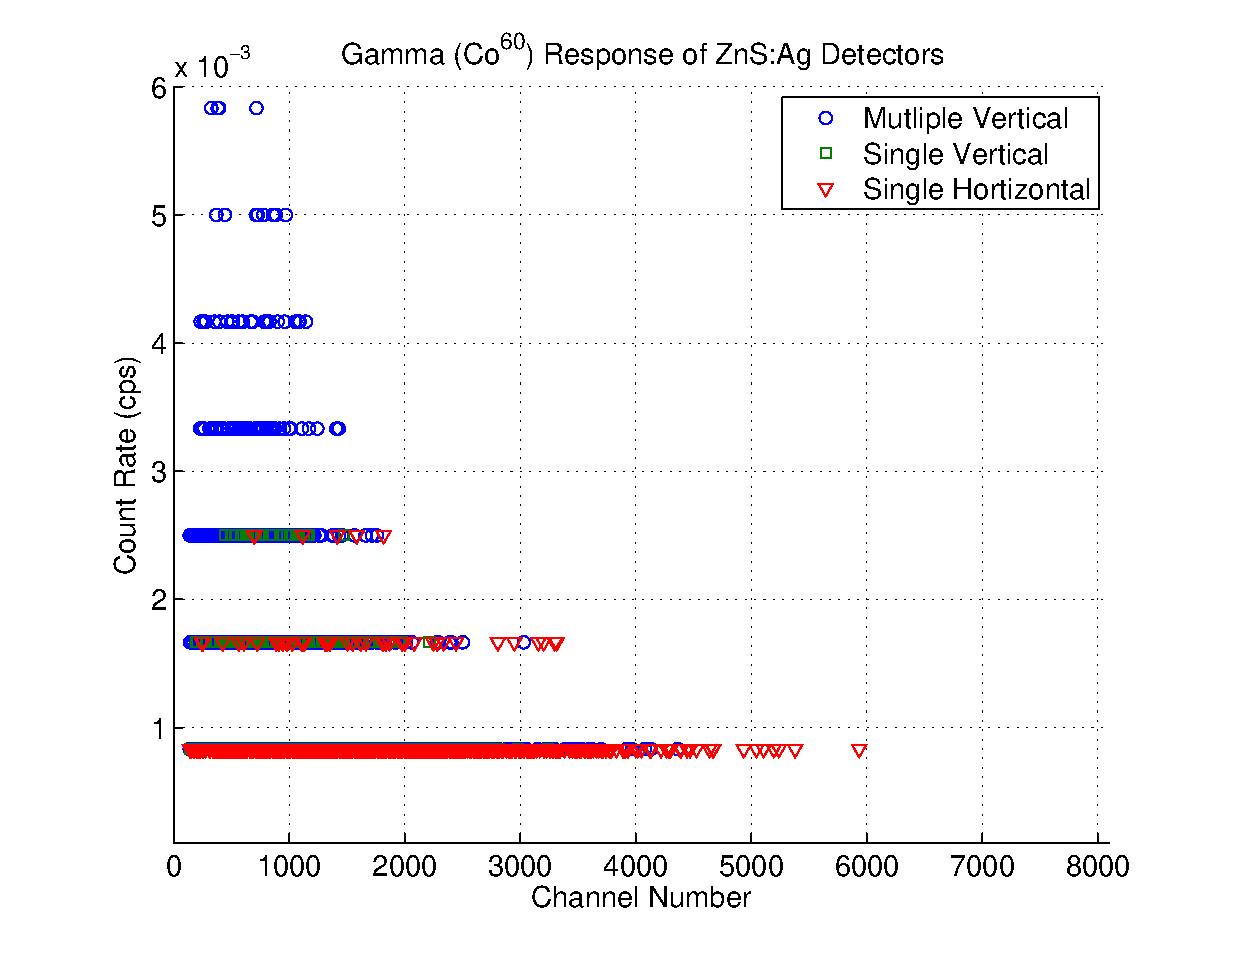
\includegraphics[width=\textwidth]{images/EJ426HD_Multi_GammaComparison.eps}
		\caption{Gamma Spectra of EJ426HD2}
	\end{figure}
\end{column}
\begin{column}{0.45\textwidth}
	\tiny
	\begin{figure}
		\centering
		\includegraphics[width=\textwidth]{images/EJ426HD_Multi_GammaIntEff.eps}
		\caption{Gamma Intrisinic Efficiency of EJ426-HD2}
\end{figure}
\end{column}
\end{columns}
\end{frame}
%%%%%%%%%%%%%%%%%%%%%%%%%%%%%%%%%%%%%%%%%%%%%%%%%%%%%%%%%%%%%%%%%%%%%%%%%%%%%%%

% !TEX TS-program = pdflatex
% !TEX encoding = UTF-8 Unicode

% Matthew Urffer Master Thesis
% 
% PSD Performance
%
\section{PSD}

%%%%%%%%%%%%%%%%%%%%%%%%%%%%%%%%%%%%%%%%%%%%%%%%%%%%%%%%%%%%%%%%%%%%%%%%%%%%%%%
%                                                                             %
%                               PSD PERFORMANCE                               %
%                                                                             %
%%%%%%%%%%%%%%%%%%%%%%%%%%%%%%%%%%%%%%%%%%%%%%%%%%%%%%%%%%%%%%%%%%%%%%%%%%%%%%%
\subsection{PS Films}
%%%%%%%%%%%%%%%%%%%%%%%%%%%%%%%%%%%%%%%%%%%%%%%%%%%%%%%%%%%%%%%%%%%%%%%%%%%%%%%
\begin{frame}{PSD Performance (PS Films I)}
\small
\begin{itemize}
	\item Enhanced performance can be achieved with PSD (theoretically)
	\item PS films show some ability for PSD
	\item None of the films are optimized \cite{zaitseva_plastic_2012}
\end{itemize}
\begin{columns}[onlytextwidth]
\begin{column}{0.30\textwidth}
	\tiny
	\begin{figure}
		\centering
		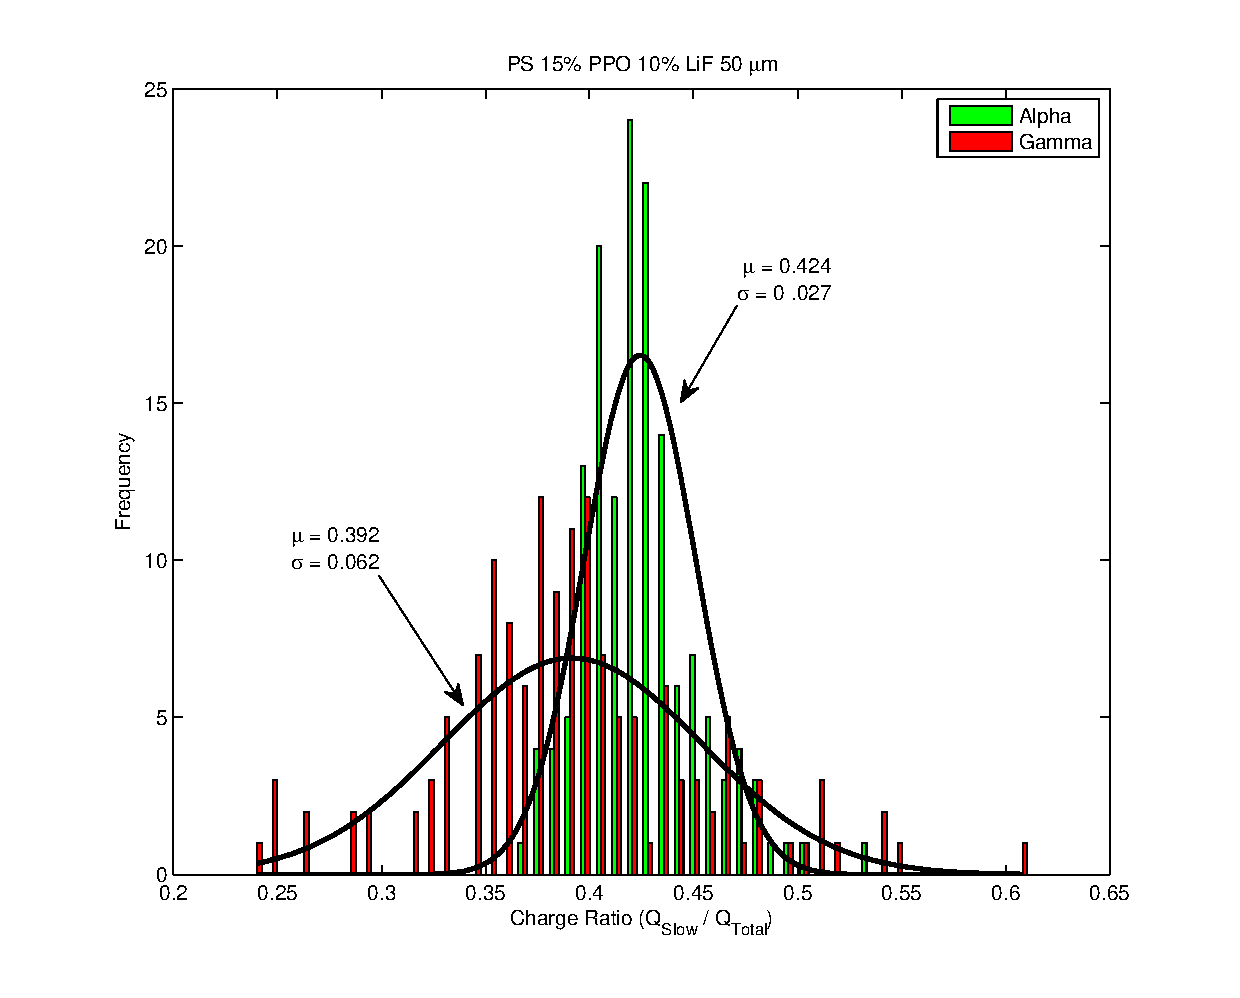
\includegraphics[width=\textwidth]{images/ChargeIntegration_PS_LiF_POP_50um.eps}
		\caption{PS 10\% LiF 50 $\mu$m}
	\end{figure}
\end{column}
\begin{column}{0.30\textwidth}
	\tiny
	\begin{figure}
		\centering
		\includegraphics[width=\textwidth]{images/ChargeIntegration_PS_LiF_POP_151um.eps}
		\caption{PS 10\% LiF 150 $\mu$m}
	\end{figure}
\end{column}
\begin{column}{0.30\textwidth}
	\tiny
	\begin{figure}
		\centering
		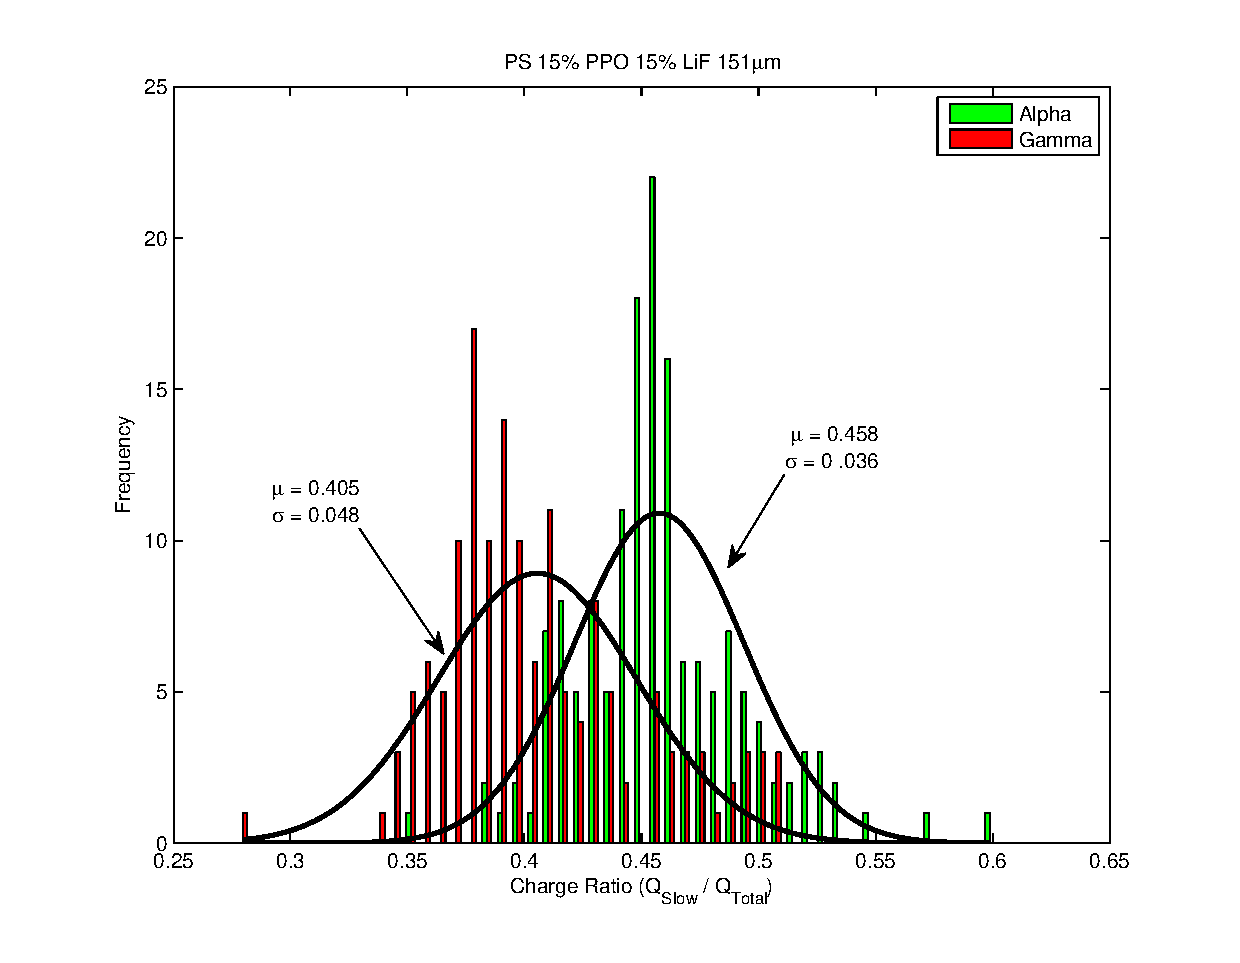
\includegraphics[width=\textwidth]{images/ChargeIntegration_PS_LiF15_POP_151um.eps}
		\caption{PS 15\% LiF 150 $\mu$m}
	\end{figure}
\end{column}
\end{columns}
\end{frame}
%%%%%%%%%%%%%%%%%%%%%%%%%%%%%%%%%%%%%%%%%%%%%%%%%%%%%%%%%%%%%%%%%%%%%%%%%%%%%%%
\begin{frame}{PSD Performance (PS Films II)}
\small
\begin{itemize}
	\item Thicker films tend to have better PSD
	\item Additional LiF decrease PSD performance
\end{itemize}
\begin{columns}[onlytextwidth]
\begin{column}{0.45\textwidth}
	\tiny
	\begin{figure}
		\centering
		\includegraphics[width=\textwidth]{images/ROC_Comparison.eps}
		\caption{ROC Curves of Charge Integration Classifier (PS Films)}
	\end{figure}
\end{column}
\begin{column}{0.45\textwidth}
	\tiny
	\begin{figure}
		\centering
		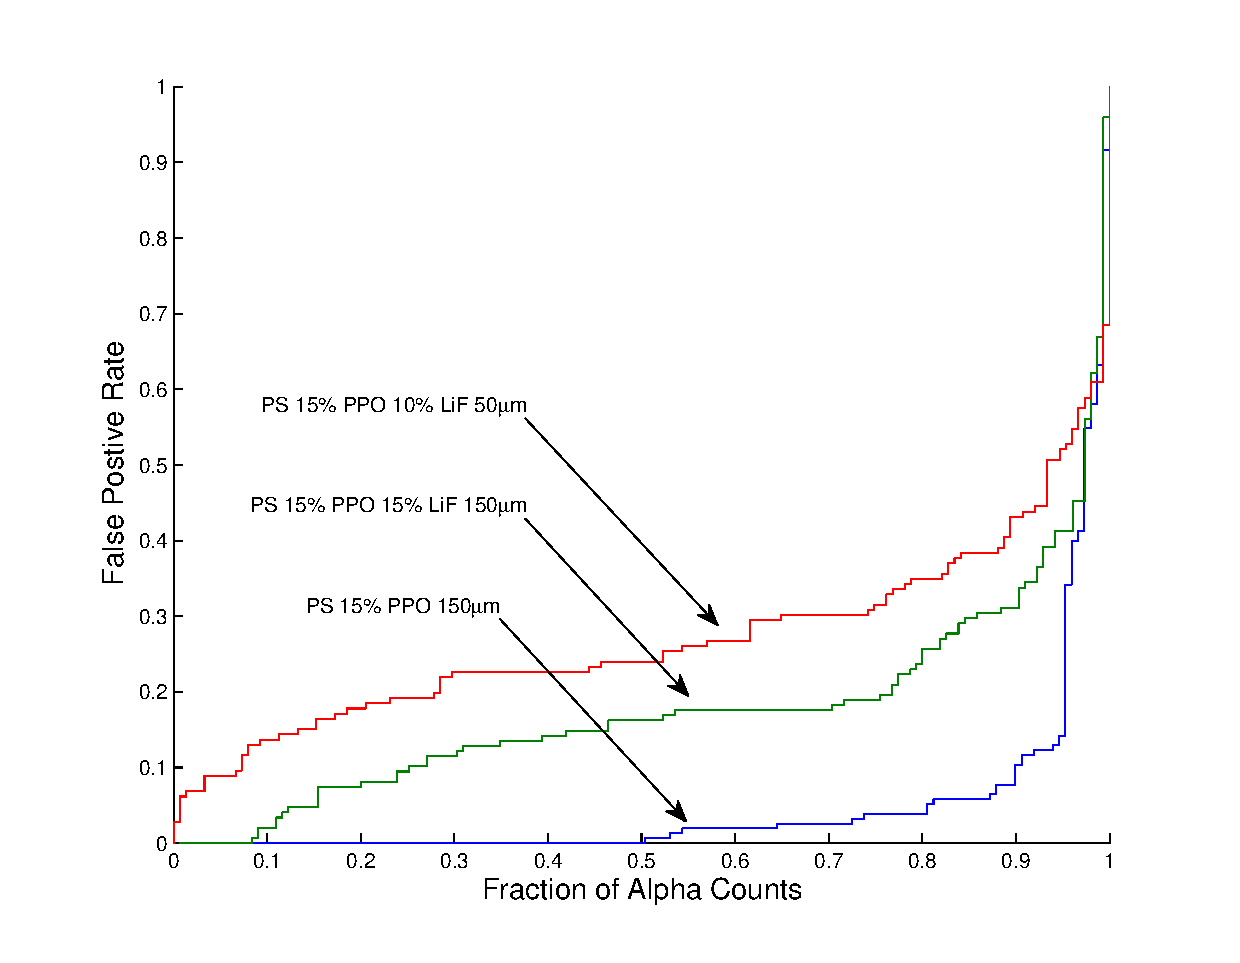
\includegraphics[width=\textwidth]{images/FPRvsFractionCounts_Comparison.eps}
		\caption{Possible Configuration}
	\end{figure}
\end{column}
\end{columns}
\end{frame}
%%%%%%%%%%%%%%%%%%%%%%%%%%%%%%%%%%%%%%%%%%%%%%%%%%%%%%%%%%%%%%%%%%%%%%%%%%%%%%%
\subsection{PEN Films}
%%%%%%%%%%%%%%%%%%%%%%%%%%%%%%%%%%%%%%%%%%%%%%%%%%%%%%%%%%%%%%%%%%%%%%%%%%%%%%%
\begin{frame}{PSD Performance (PEN Films)}
\tiny
\begin{itemize}
	\item PEN films demonstrated little capability for PSD
	\item PEN films where mounted on Katpon, which scintillates
	\item None of the films are optimized \cite{zaitseva_plastic_2012}
\end{itemize}
	\begin{figure}
		\centering
		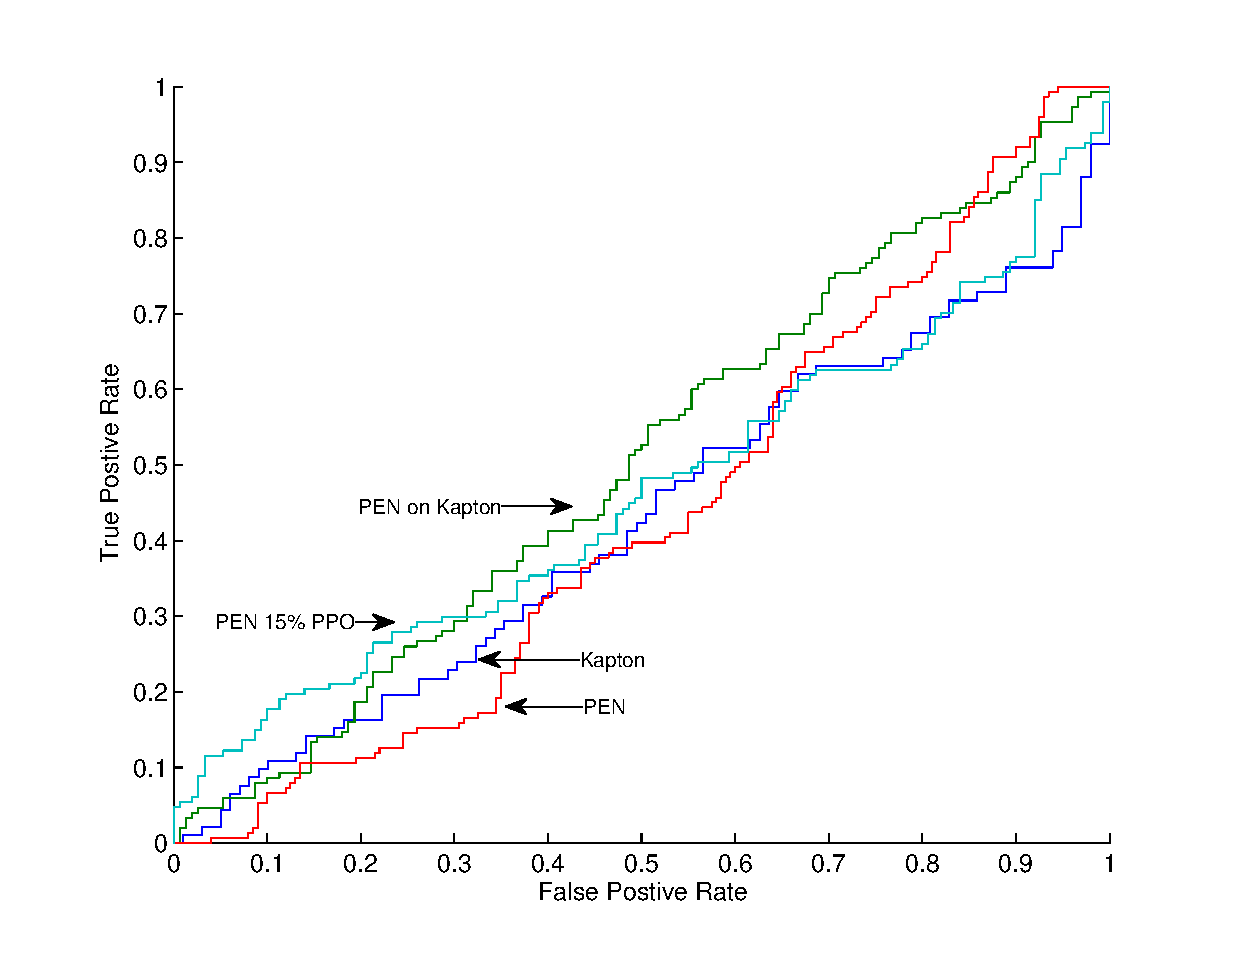
\includegraphics[height=0.55\textheight]{images/PEN_ROC_Comparison.eps}
		\caption{ROC Curves of Charge Integration Classifier (PEN Films)}
	\end{figure}
\end{frame}

\section*{Conclusions}
%%%%%%%%%%%%%%%%%%%%%%%%%%%%%%%%%%%%%%%%%%%%%%%%%%%%%%%%%%%%%%%%%%%%%%%%%%%%%%%
\begin{frame}{Measurement and Data Analysis}
	\begin{itemize}
		\item A protocol has been developed for measurements
		\begin{itemize}
			\item Verification of instrument gains
			\item Neutron Measurements
			\item Gamma Measurements
			\item Various button sources
		\end{itemize}
		\item Ability to calculate MLLD necessary for $\epsilon_{int,\gamma} \le 10^{-6}$
		\item Ability to calculate light yield
	\end{itemize}
\end{frame}
%%%%%%%%%%%%%%%%%%%%%%%%%%%%%%%%%%%%%%%%%%%%%%%%%%%%%%%%%%%%%%%%%%%%%%%%%%%%%%%
\begin{frame}{Modeling}
	\begin{itemize}
		\item MCNPX modeling has been employed
		\begin{itemize}
			\item Determination of 10 mR/hr field
			\item Determination of film performance to neutrons
			\begin{itemize}
				\item Neutron Irridiator
				\item Mock up of DHS/DNDO test configuration
			\end{itemize}
		\end{itemize}
		\item Future work will be completed with GEANT4
	\end{itemize}
\end{frame}
%%%%%%%%%%%%%%%%%%%%%%%%%%%%%%%%%%%%%%%%%%%%%%%%%%%%%%%%%%%%%%%%%%%%%%%%%%%%%%%
\begin{frame}{Summary}

  \begin{itemize}
  \item
    A framework has been developed for the characterization of possible replacement technologies for radiation portal monitors
  \item
    A framework has been developed for pulse shape discrimination 
  \item
    Thin polymeric films have been demonstrated to have the necessary interaction rates for radiation portal monitors
  \end{itemize}
	\centering
		\includegraphics[width=0.5\textwidth]{images/Questions.eps}
\end{frame}

%%%%%%%%%%%%%%%%%%%%%%%%%%%%%%%%%%%%%%%%%%%%%%%%%%%%%%%%%%%%%%%%%%%%%%%%%%%%%%%
% BILBIOLGRAPHY
\begin{frame}[plain,allowframebreaks]
\frametitle{Works Cited}
	\tiny
    \bibliography{Zotero}
\end{frame}

% APPENDIX
\appendix
\section<presentation>*{\appendixname}
\subsection<presentation>*{Fundamental Physics}
\begin{frame}{Absorption Cross Sections}
\begin{figure}
	\centering
		\includegraphics[width=0.9\textwidth]{images/CrossSections.eps}
	\caption{Cross sections of selected isotopes \protect \cite{nist_neutron_2012}}
	\label{fig:CrossSections}
\end{figure}

\end{frame}




\end{document}


